\section{System overview}\label{sec:system_overview}
%{\color{green}
A da Vinci robot with connected EndoWrists has four arms with 6 - 7 actuated Degrees Of Freedom (DOF) each. Each arm has its own drivers and an embedded system controlling it. %\textcolor{red}{The embedded systems receive the desired position of the end-effector from the console from which the surgeon operates.}
The surgeon sends the commands to the embedded system by controlling the console.

As mentioned in Section \ref{sec:introduction}, the EndoWrist is highly nonlinear and constitute most of the challenge in the modelization of one arm of the robot, thus, if the force feedback can effectively be applied to the tool, it can be extended to the arm. As each arm is independent, the system designed for one arm can be extended to the full arm, the same applies to the tool. The setup used in the present project only controls one EndoWrist which has 4 DOF and is further described in Section \ref{sec:EndoWrist}.%\color{red}{As each arm is independent, the system designed for one arm can be extended to the full robot. This paper will focus on implementing a force feedback on one EndoWrist.} \\ 
 To control the EndoWrist, the embedded system of the robot is used. On a da Vinci robot the surgeon performs the operation from a console that communicates with the robot. The manipulators for the robot do not implement an interface for haptic feedback, thus, a haptic device, a Geomagic Touch (GT), is used in this setup instead of the device used on the official console. This device is further described in Section \ref{sec:Geomagic_touch}.\\
As force estimation requires computational power and an interface is required to exchange information between GT and embedded system, a computer is added to the system and connected to both devices using Ethernet cables. The entire setup is represented in Fig. \ref{fig:full_setup}
\begin{figure}[h]
\centering
\scalebox{0.97}{
\begin{tikzpicture}
        \node [box] (Geomagic) {\small{Geomagic Touch}};
        \node [box, right of=Geomagic, node distance = 3.4cm] (Computer) {Computer};
        \node [box, below of=Computer, node distance=3.3cm] (Sbrio) {Embedded\\System};
        \node [box, left of=Sbrio, node distance=2.5cm] (Driver) {Motor driver};
        \node [box, left of=Driver, node distance=2.5cm] (EndoWrist) {EndoWrist};
        % We draw an edge between the controller and system block to
        % calculate the coordinate u. We need it to place the measurement block.
        \draw [<->] (Geomagic) -- node {} (Computer);
        \draw [<->] (Computer) -- node {} (Sbrio);    
        % \draw [<->] (Geomagic) -- node[label=above:\small{UDP}] {} (Computer);
        % \draw [<->] (Computer) -- node [label=right:\small{UDP}] {} (Sbrio);
        \draw [<->] (Sbrio) -- node {} (Driver);
        \draw [->] (Driver) -- node {} (EndoWrist);
        
        \draw[thick,dashed] ($(-1.5,1)+(Geomagic)$) -- ($(1.5,1)+(Computer)$) -- ($(1.5,-1)+(Computer)$) -- ($(-1.5,-1)+(Geomagic)$)-- ($(-1.5,1)+(Geomagic)$);
        \draw[thick,dashed] ($(-1.5,1)+(EndoWrist)$) -- ($(1.5,1)+(Sbrio)$) -- ($(1.5,-1)+(Sbrio)$) -- ($(-1.5,-1)+(EndoWrist)$)-- ($(-1.5,1)+(EndoWrist)$);
        
        \node at (2,1.4) {\textbf{Console}};
        \node at (1.5,-2) {\textbf{da Vinci robot}};
\end{tikzpicture}
}
\caption{Block diagram representing the system.}
\label{fig:full_setup}
\end{figure}
%}


%{\color{red}
%\subsection{Entire setup}

%A fully featured da Vinci robot with connected EndoWrists has four arms with 6 - 7 actuated DOF each.
%However, for test purposes, a small scale setup for controlling one EndoWrist has been created, see figure \ref{fig:Mec_d}.

%\begin{figure}
%    \centering
%    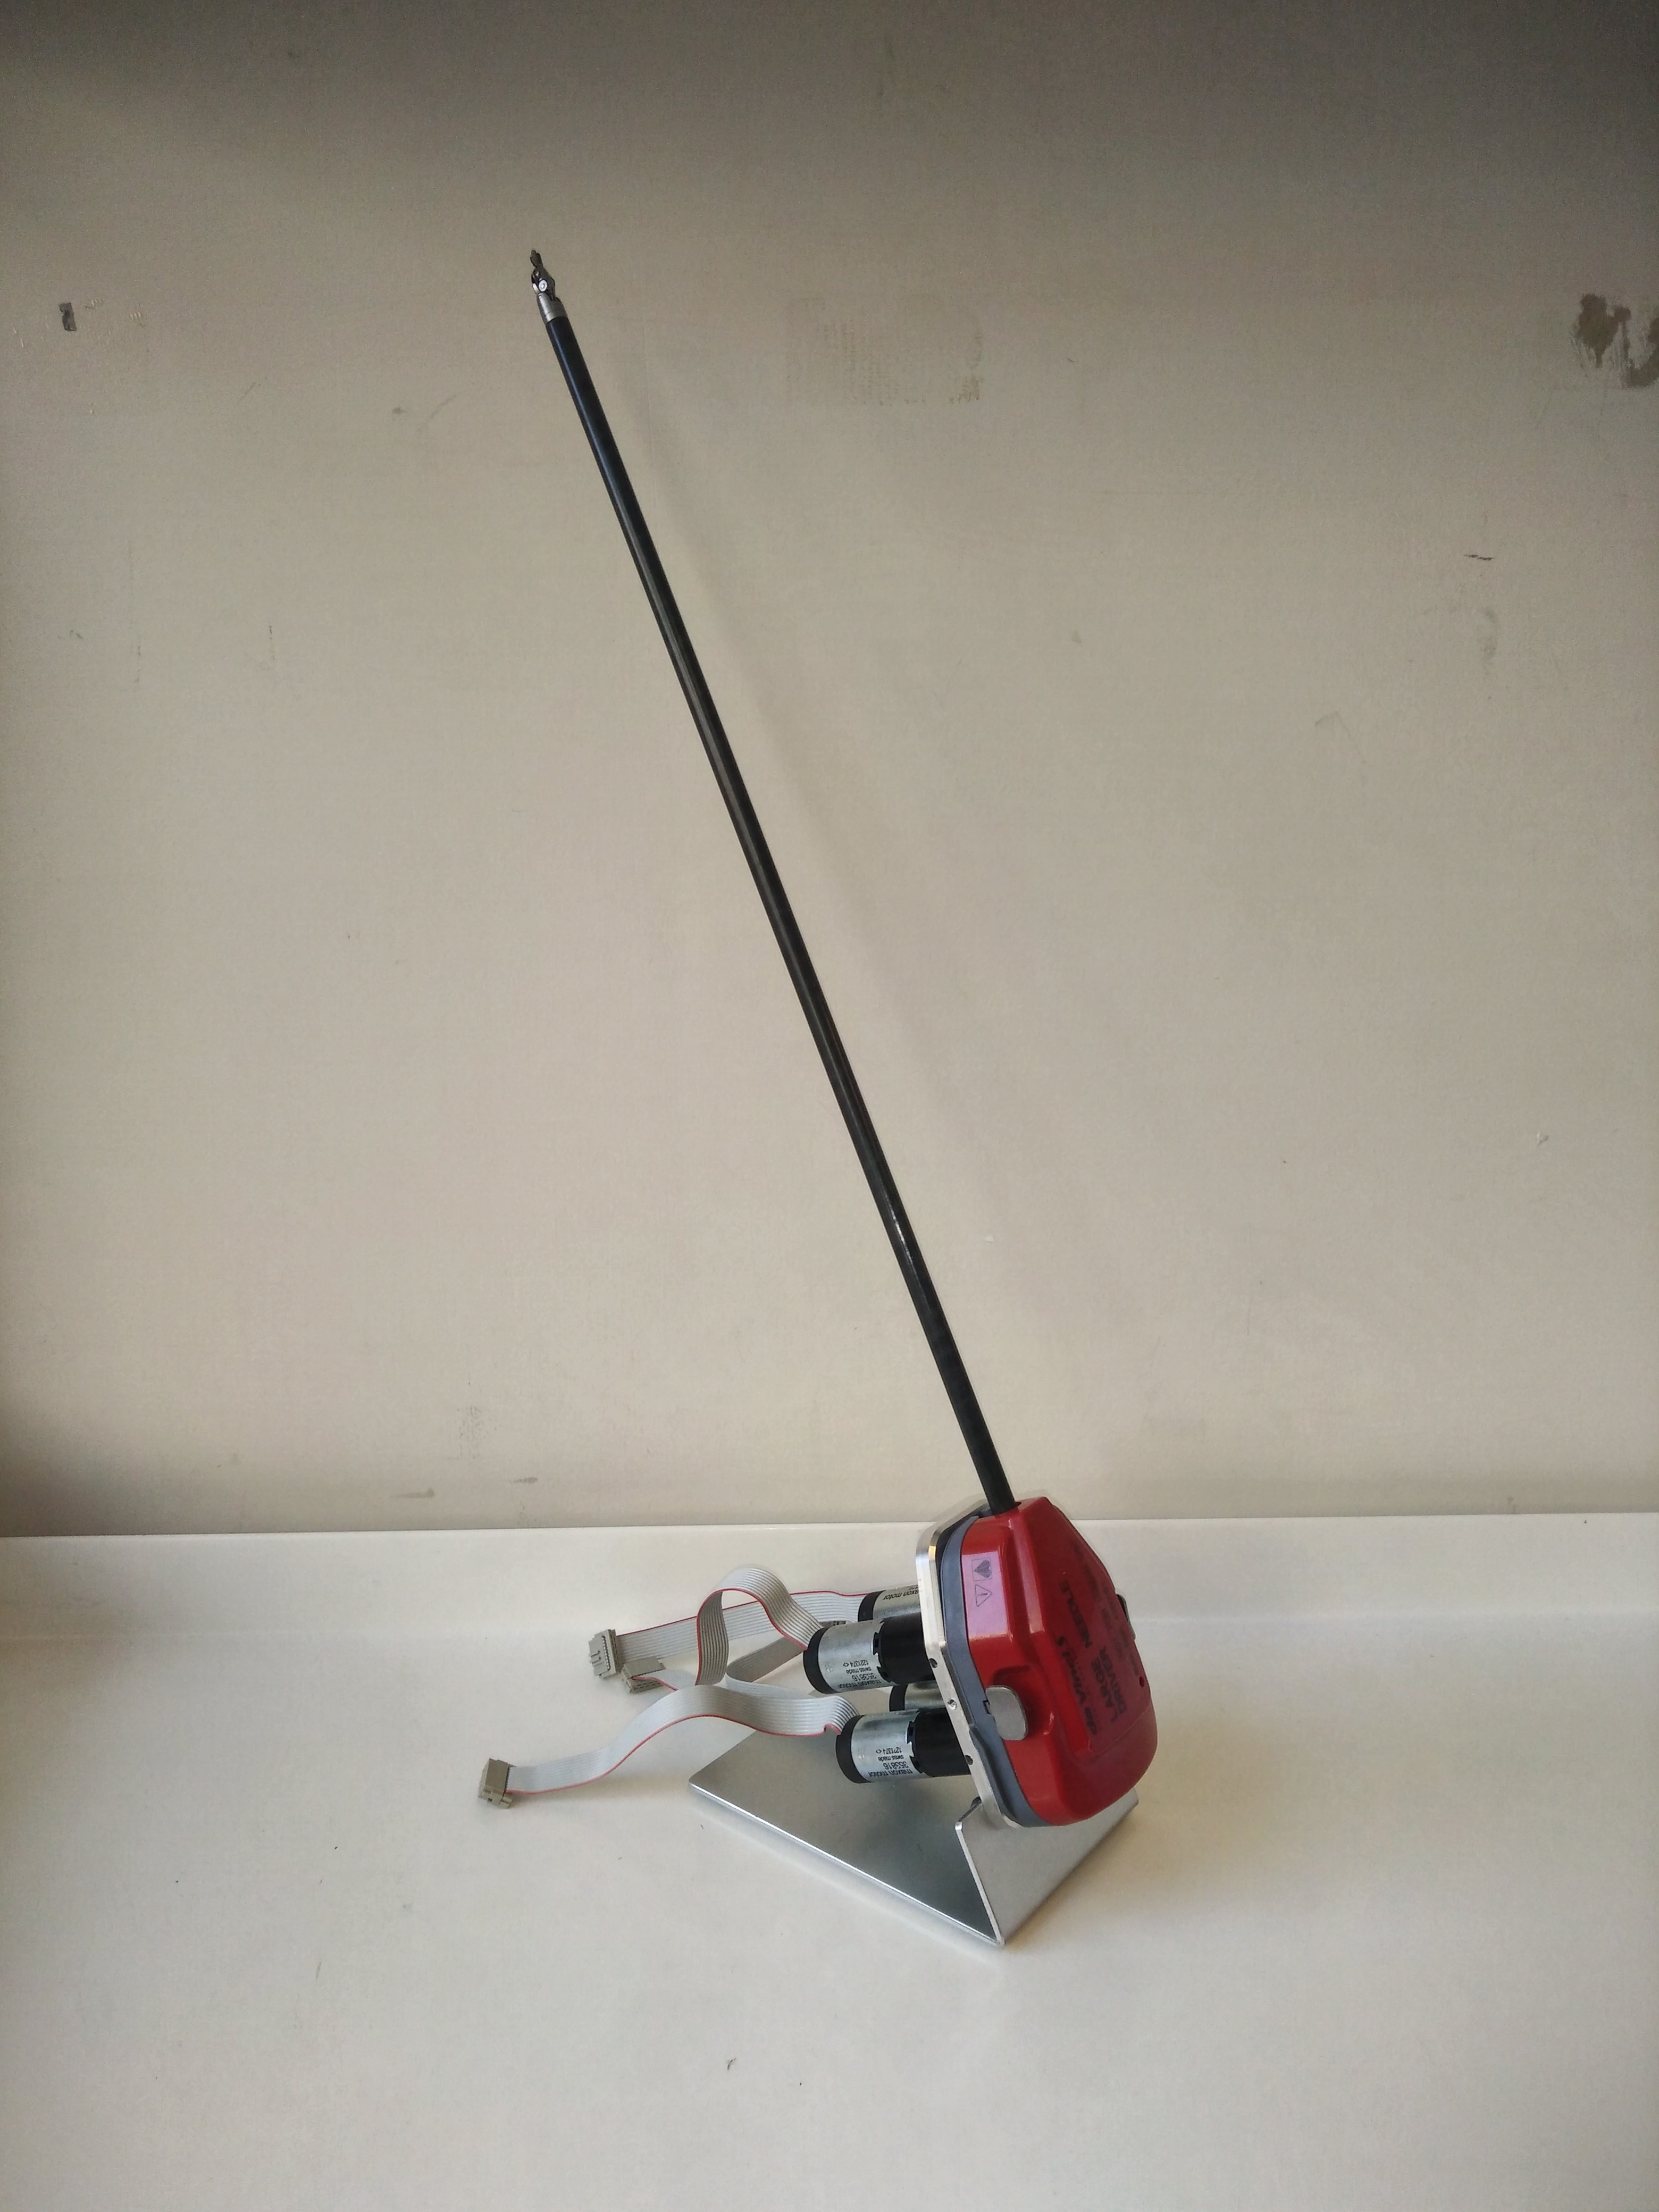
\includegraphics[width=0.4\linewidth]{Test_setup4.jpg}
%    \caption{Full view of the mechanical test setup}
%    \label{fig:Mec_d}
%\end{figure}

%Representing the onboard computer on the da Vinci robot, an sbRIO board has been implemented to control the test setup. 
%In order to perform higher level functions, such as force feedback control, it is necessary to remotely handle data and send high-level commands.
%This is handled by an external computer system. %that is connected to the Geomagic touch.

%The sbRIO board communicates with the computer using User Datagram Protocol (UDP), while the Geomagic Touch, see section \ref{sec:Geomagic_touch}, does so using TCP/IP.
% The computer performs force estimation using a dynamical model of the test setup (or EndoWrist, more precisely), this is vital for force feedback.
% In order to connect software components responsible for communicating with hardware and the ones responsible for the control algorithm and estimation, the Robot Operating System (ROS) is used.
% ROS uses a network architecture to share data between components via data streams.





% \begin{figure}[h]
% \centering
% \scalebox{0.97}{
% \begin{tikzpicture}
%     % We start by placing the blocks
%     \node [box] (Geomagic) {\small{Geomagic Touch}};
%     \node [box, right of=Geomagic, node distance = 3.4cm] (ROS) {ROS};
%     \node [box, right of=ROS, node distance=3.3cm] (DaVinci) {da Vinci};
%     % We draw an edge between the controller and system block to
%     % calculate the coordinate u. We need it to place the measurement block.
%     \draw [<->] (Geomagic) -- node[label=above:\small{TCP/IP}] {} (ROS);
%     \draw [<->] (ROS) -- node [label=above:\small{UDP}] {} (DaVinci);
% \end{tikzpicture}
% }
% \caption{Block diagram representing the system.}
% \end{figure}


% In our proposed system, the surgeon uses the Geomagic Touch joystick to control an EndoWrist tool on one of the arms of the da Vinci surgical robot.
% It is important for the operator to have a feeling of the resistance the tool is experiencing in order to adjust the position and grip strength and thus prevent damage to the patient's tissue.
% In order to project the reaction forces acting on the EndoWrist to the operator, we use the Geomagic Touch haptic feedback feature. The communication between the da Vinci robot, the Geomagic Touch and the controller is done through Robots Operating System (ROS).

% }

\subsection{Geomagic touch}\label{sec:Geomagic_touch}
The Geomagic Touch is a haptic feedback device, which has the ability to actuate its joints in such a way that the user feels resistance when moving the pen. 


\begin{figure}[h]
  \centering
  \begin{subfigure}{.22\textwidth}
    \centering
    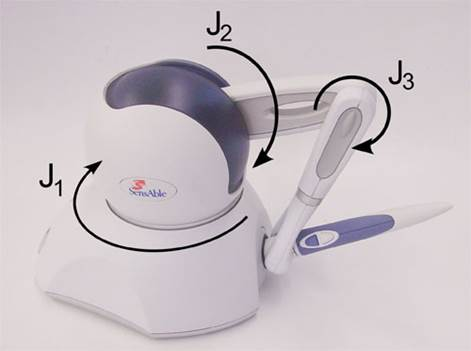
\includegraphics[width=\linewidth]{haptick1.png}
    \caption{Overview of the Geomagic Touch's first three joints.}
    \label{fig:phantom1}
  \end{subfigure}
  \begin{subfigure}{.22\textwidth}
    \centering
    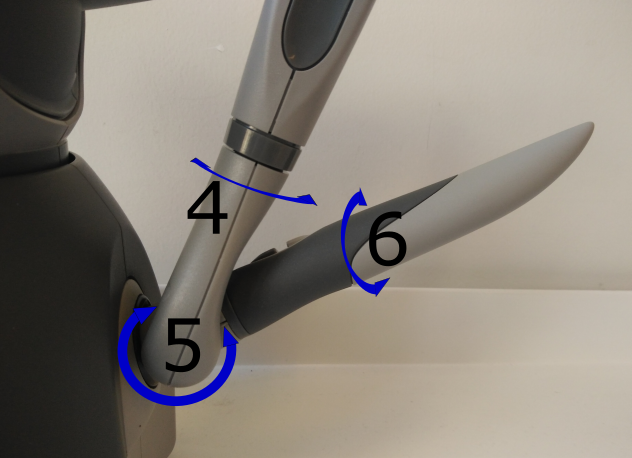
\includegraphics[width=\linewidth]{haptick2.png}
    \caption{Overview of the Geomagic Touch's last three joint}
    \label{fig:phantom2}
  \end{subfigure}
\caption{Overview of all the Geomagic Touch's joints.}
\label{fig:phantom_omni}
\end{figure}


On Fig. \ref{fig:phantom_omni}, it can be seen that the Geomagic Touch has six DOF, where the first three can be actuated, see Fig. \ref{fig:phantom1}. This means that the device has the ability to generate force feedback with three translational DOF, in this case corresponding to the EndoWrist's roll, pitch and yaw movements.



    
\subsection{EndoWrist}\label{sec:EndoWrist}

%{\color{green}
An EndoWrist, see Fig. \ref{fig:Endo_plates}, is a surgical tool for the da Vinci robot which can be manipulated \textcolor{green}{in a similar manner} as a human wrist. It provides the surgeon the ability to operate with the robot as the operator would without it. To replicate the movements of a human wrist, the tool is composed of a system of cables and pulleys. This construction imitates the human tendons however it also introduces nonlinearities in the tool, and thus, a challenge for controlling or modeling it.

\begin{figure}[h]
  \centering
  \begin{subfigure}{.22\textwidth}
    \centering
    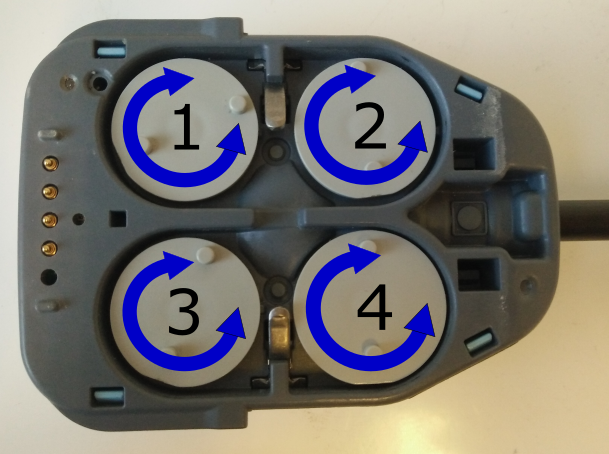
\includegraphics[height=0.55\linewidth,]{Endowrist22.png}
    \caption{Actuator plates, which can manipulate the end effector position}
    \label{fig:Endo_plates}
  \end{subfigure}
  \begin{subfigure}{.22\textwidth}
    \centering
    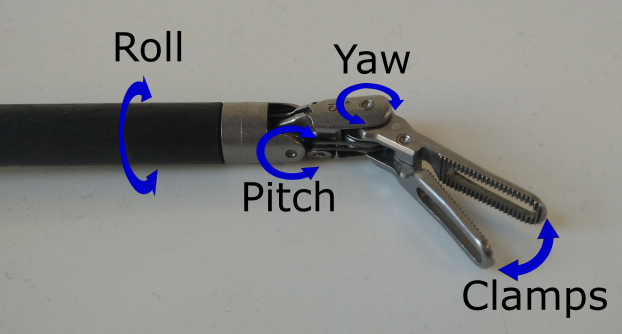
\includegraphics[height=0.55\linewidth]{Endowrist31.png}
    \caption{End-effector of the EndoWrist\newline}
    \label{fig:Endo_end}
  \end{subfigure}
\caption{The EndoWrist and its end-effector}
\label{fig:endowrits_set}
\end{figure}

In real operation, each arm has six to seven actuated DOF in total, however, the EndoWrist itself, when disconnected from the robot, only has four DOF. Each DOF is actuated through a plate, see Fig. \ref{fig:Endo_plates}. The four DOF are roll, pitch, yaw and clamp, see Fig. \ref{fig:Endo_end}. The nonlinearities of the tool are analysed when building the model in Section \ref{sec:force_estimation}.
%}

% {\color{red}An EndoWrist, see Figure \ref{fig:Endo_plates}, is a surgical tool which can be manipulated as a human wrist.
% It is used in surgical procedures such as Laparoscopic surgeries,  where small incisions in the human body is made during the surgery.
% Because the incision cuts are small, blood loss during the surgery and the risk of infection is reduced. This has a positive effect on the recovery time of the patient\cite{RIGSP}.


% \begin{figure}[h]
%   \centering
%   \begin{subfigure}{.22\textwidth}
%     \centering
%     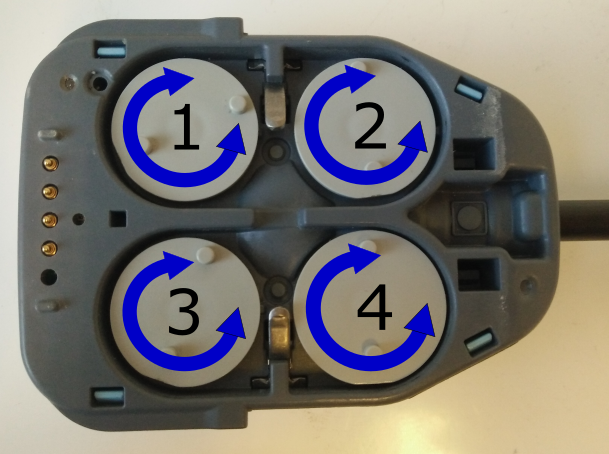
\includegraphics[width=\linewidth,]{Endowrist22.png}
%     \caption{Actuator plates, which can manipulate the end effector position}
%     \label{fig:Endo_plates}
%   \end{subfigure}
%   \begin{subfigure}{.22\textwidth}
%     \centering
%     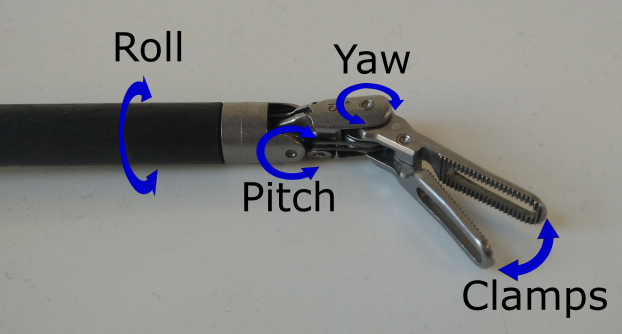
\includegraphics[width=\linewidth]{Endowrist31.png}
%     \caption{End-effector of the EndoWrist\newline}
%     \label{fig:Endo_end}
%   \end{subfigure}
% \caption{The EndoWrist and its end-effector}
% \label{fig:endowrits_set}
% \end{figure}


% The EndoWrist can be manipulated as a human wrist with two clamps, thus having four degrees of freedom (DOF), see Figure \ref{fig:Endo_end}. This gives the movement of roll, pitch, yaw and an opening/closing mechanism that acts as the thumb and index finger of a hand.


% The end-effector is manipulated by the four wheels seen on Figure \ref{fig:Endo_plates}. The EndoWrist is cable driven, which provides the opportunity of making it small but also makes the system nonlinear due to dry friction.}



% In out\todo{our?} proposed system, the surgeon uses the Geomagic Touch joystick to control an Endowrist tool on one of the arms of the DaVinci surgical robot.
% It is important for the operator to have a feeling of resistance the tool is experiencing in order to adjust the position and grip strength and thus prevent damage to the patients tissue.
% To achieve this, we use the Geomagics haptic feedback feature in order to project the reaction forces acting on the Endowrist to the operator. 
% The communication between system components is done through the Robot Operating System (ROS).

% \subsection{Endowrist}
% An Endowrist, see \ref{fig:Endo_plates} \todo{figref?} is a surgical tool which can be manipulated as a human wrist. 
% It is used in surgical procedures such as Laparoscopic surgeries, better known as minimally invasive surgery (MIS), where small incisions in the human body is made during the surgery. 
% Because the incision cuts are small, blood lose\todo{blood loss?} during the surgery and the risk of infection is reduced. This has a positive effect on the recovery time for the patient.

% \begin{figure}
%   \centering
%   \begin{subfigure}{.22\textwidth}
%     \centering
%     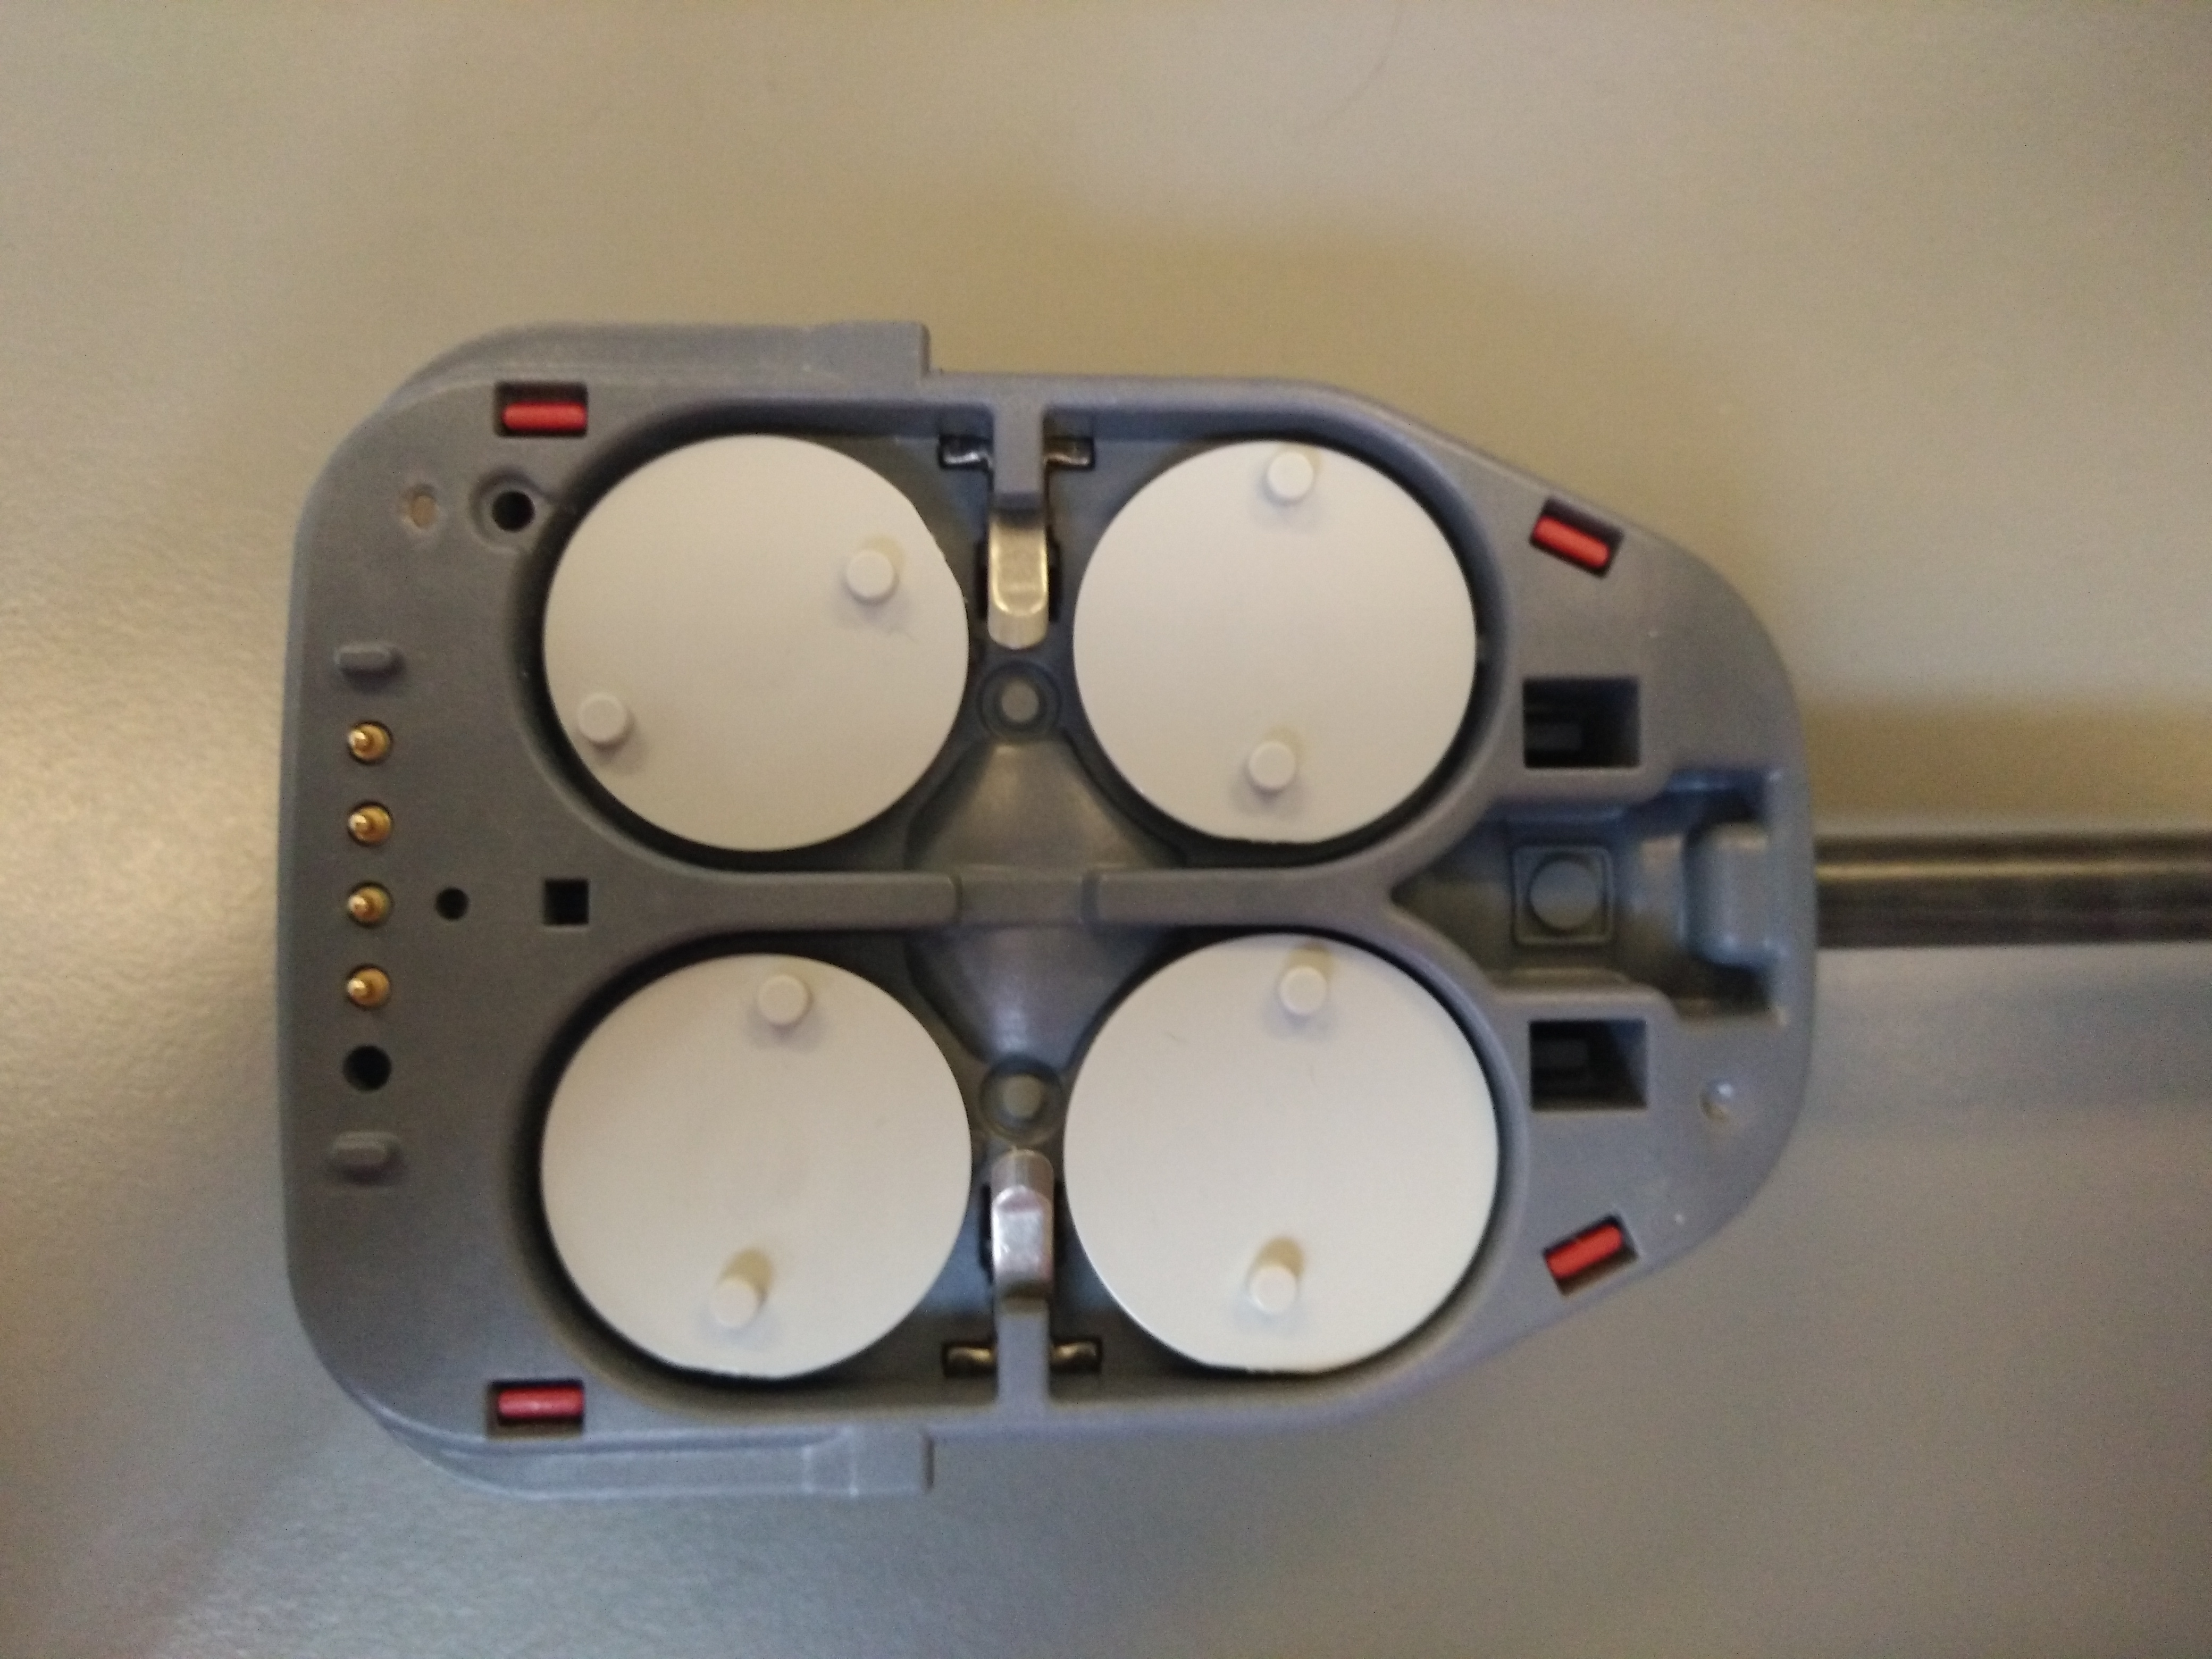
\includegraphics[width=\linewidth]{Endowrist2.jpg}
%     \caption{Actuator plates, which can alternate the end effector position}
%     \label{fig:Endo_plates}
%   \end{subfigure}
%   \begin{subfigure}{.22\textwidth}
%     \centering
%     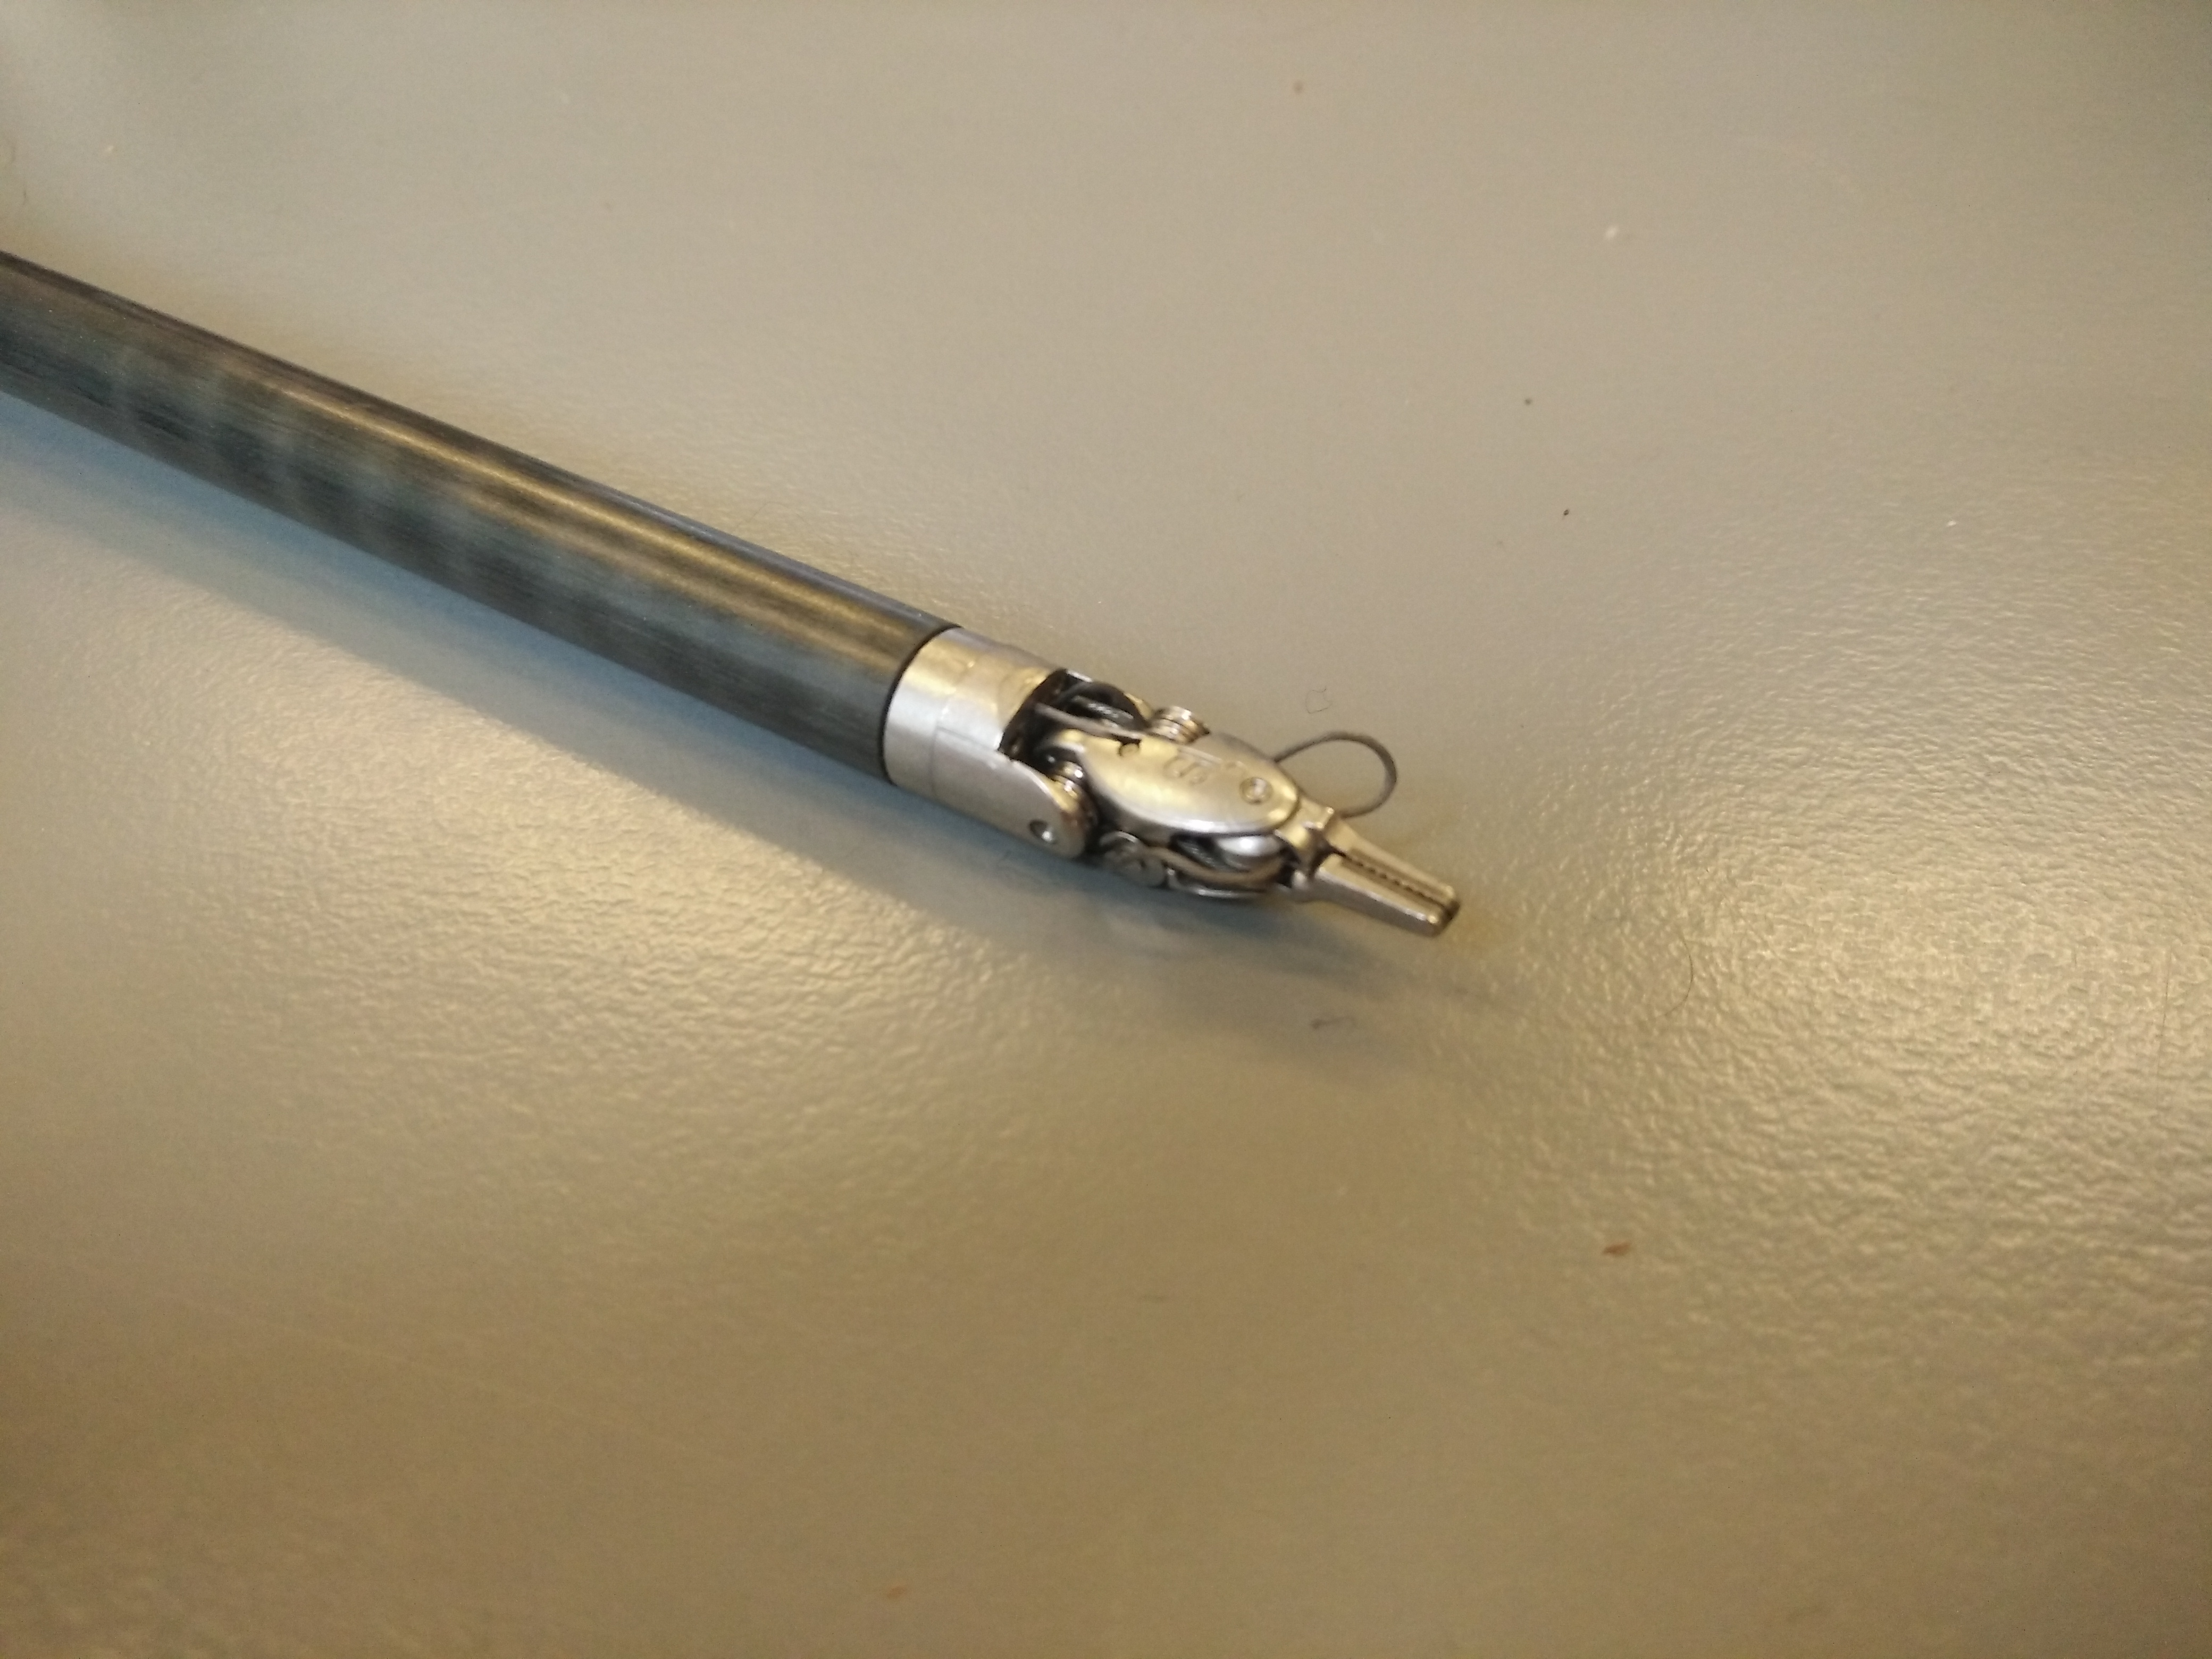
\includegraphics[width=\linewidth]{Endowrist3.jpg}
%     \caption{End effector of the Endowrist\newline}
%     \label{fig:Endo_end}
%   \end{subfigure}
% \caption{The Endowrist and it's end-effector}
% \label{fig:endowrits_set}
% \end{figure}

% As mentioned the Endowrist has the ability to be manipulated as a human wrist and thereby has four DOF, see \ref{fig:Endo_end}\todo{1b doesn't really show the 4DOF}\todo{figref}. This enables the movement of roll, pitch, yaw and an open closing mechanism that acts as the thumb and index finger of a hand. 

% The end-effector is manipulated by the four wheels seen on \ref{fig:Endo_plates}. Wheel one and three define the movement of the yaw and the closing mechanism. Wheel two and four moves the pitch and roll. The Endowrist is cable driven, which enables the opportunity of making the Endowrist small but it also makes the system nonlinear as the force acting at one end is not directly transmitted to the other end due to friction. 

% \subsection{Geomagic touch}
% The geomagic touch is a haptic feedback device, which has the ability to manipulate its joints in such a way that the user feels resistance when moving the pen in a certain direction or way. 
% The geomagic touch described in this section is the model Phantom omni and can be seen on \ref{fig:phantom_omni}.

% \begin{figure}
%   \centering
%   \begin{subfigure}{.22\textwidth}
%     \centering
%     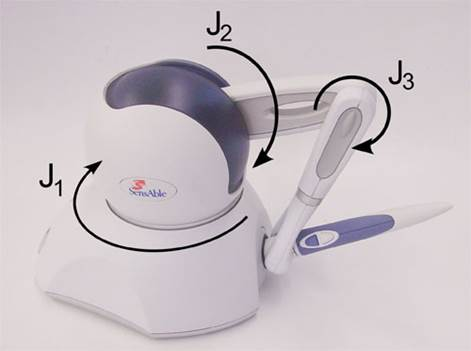
\includegraphics[width=\linewidth]{haptick1.jpg}
%     \caption{Overview of the Phantom omni's first three joints.}
%     \label{fig:phantom1}
%   \end{subfigure}
%   \begin{subfigure}{.22\textwidth}
%     \centering
%     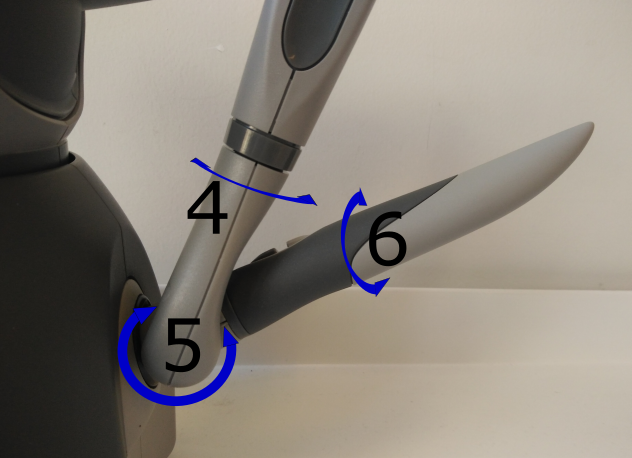
\includegraphics[width=\linewidth]{haptick2.png}
%     \caption{Overview of the Phantom omni's last three joint}
%     \label{fig:phantom2}
%   \end{subfigure}
% \caption{Overview of all the Phantom omni's joints\cite{phantom_omni}}
% \label{fig:phantom_omni}
% \end{figure}

% As mentioned the Phantom omni has the ability to generate resistance for the user. In other words, when moved in a specific direction it can create a counter force in respect to a certain position. On \ref{fig:phantom_omni}, it can be seen that the omni has six DOF, where only the first three can be actuated, see \ref{fig:phantom1}. This means that the device only has the ability to generate force feedback with three DOF, in this case roll, pitch and yaw.

% The connection to the omni can either be made directly through a ethernet cable or through ethernet cable to a usb converter into a computer. For programming the omni an API is included, which enables the connection to the omni. The Geomagic Touch has a lot of features which can be programmed through the language C++, e.g force rendering or drawing graphics.

% \subsection{ROS} \todo{we should not describe what ROS is}
% The ROS is an open source software development tool for implementing robotics software. It provides the opportunity of hardware abstraction, low level device control, implementation of commonly used functionalities, messages between different processes and package management.%{\cite{wiki_ros}}
%  It provides tools and libraries which utilize the the opportunity of communicating between disturbed computers, obtaining, writing and running codes.
 
% ROS has three different levels of concepts\cite{Wiki_ros_concepts}

% \begin{itemize}
% \item \textbf{The file system level}

% Handles the main unit for a ROS system which is packages. A package may include data sets, ROS dependent libraries, configure files etc. to define a ROS process. In ROS a process is denoted as a node. 
% \item \textbf{The computation graph level}

% Handles the communication of the peer to peer network of the system in which data is processed. Through the computation graph level, the different nodes can communicate with each other by messages. When a node is sending data it is said to be publishing a topic. The different nodes can then subscribe to this topic to get the information that is published.
% \item \textbf{The Community level}

% ROS has a huge community which contain distribution of software installations, repositories and documentation of ROS. It also has a question and answer section with ROS related topics.
% This community makes the process of learning the system considerably easier.
% \end{itemize}

% \subsection{Overview}
% As mentioned before , a fully featured DaVinci robot \todo{arm} has 7 degrees of freedom on the Endowrist instrument.
% Since the robot has 4 arms, there are 4 instruments.
% Although our setup controls only 4 motors, in funcionality it is equivalent to one DaVinci arm. \todo{I find this confusing}

% \begin{figure}
%     \centering
%     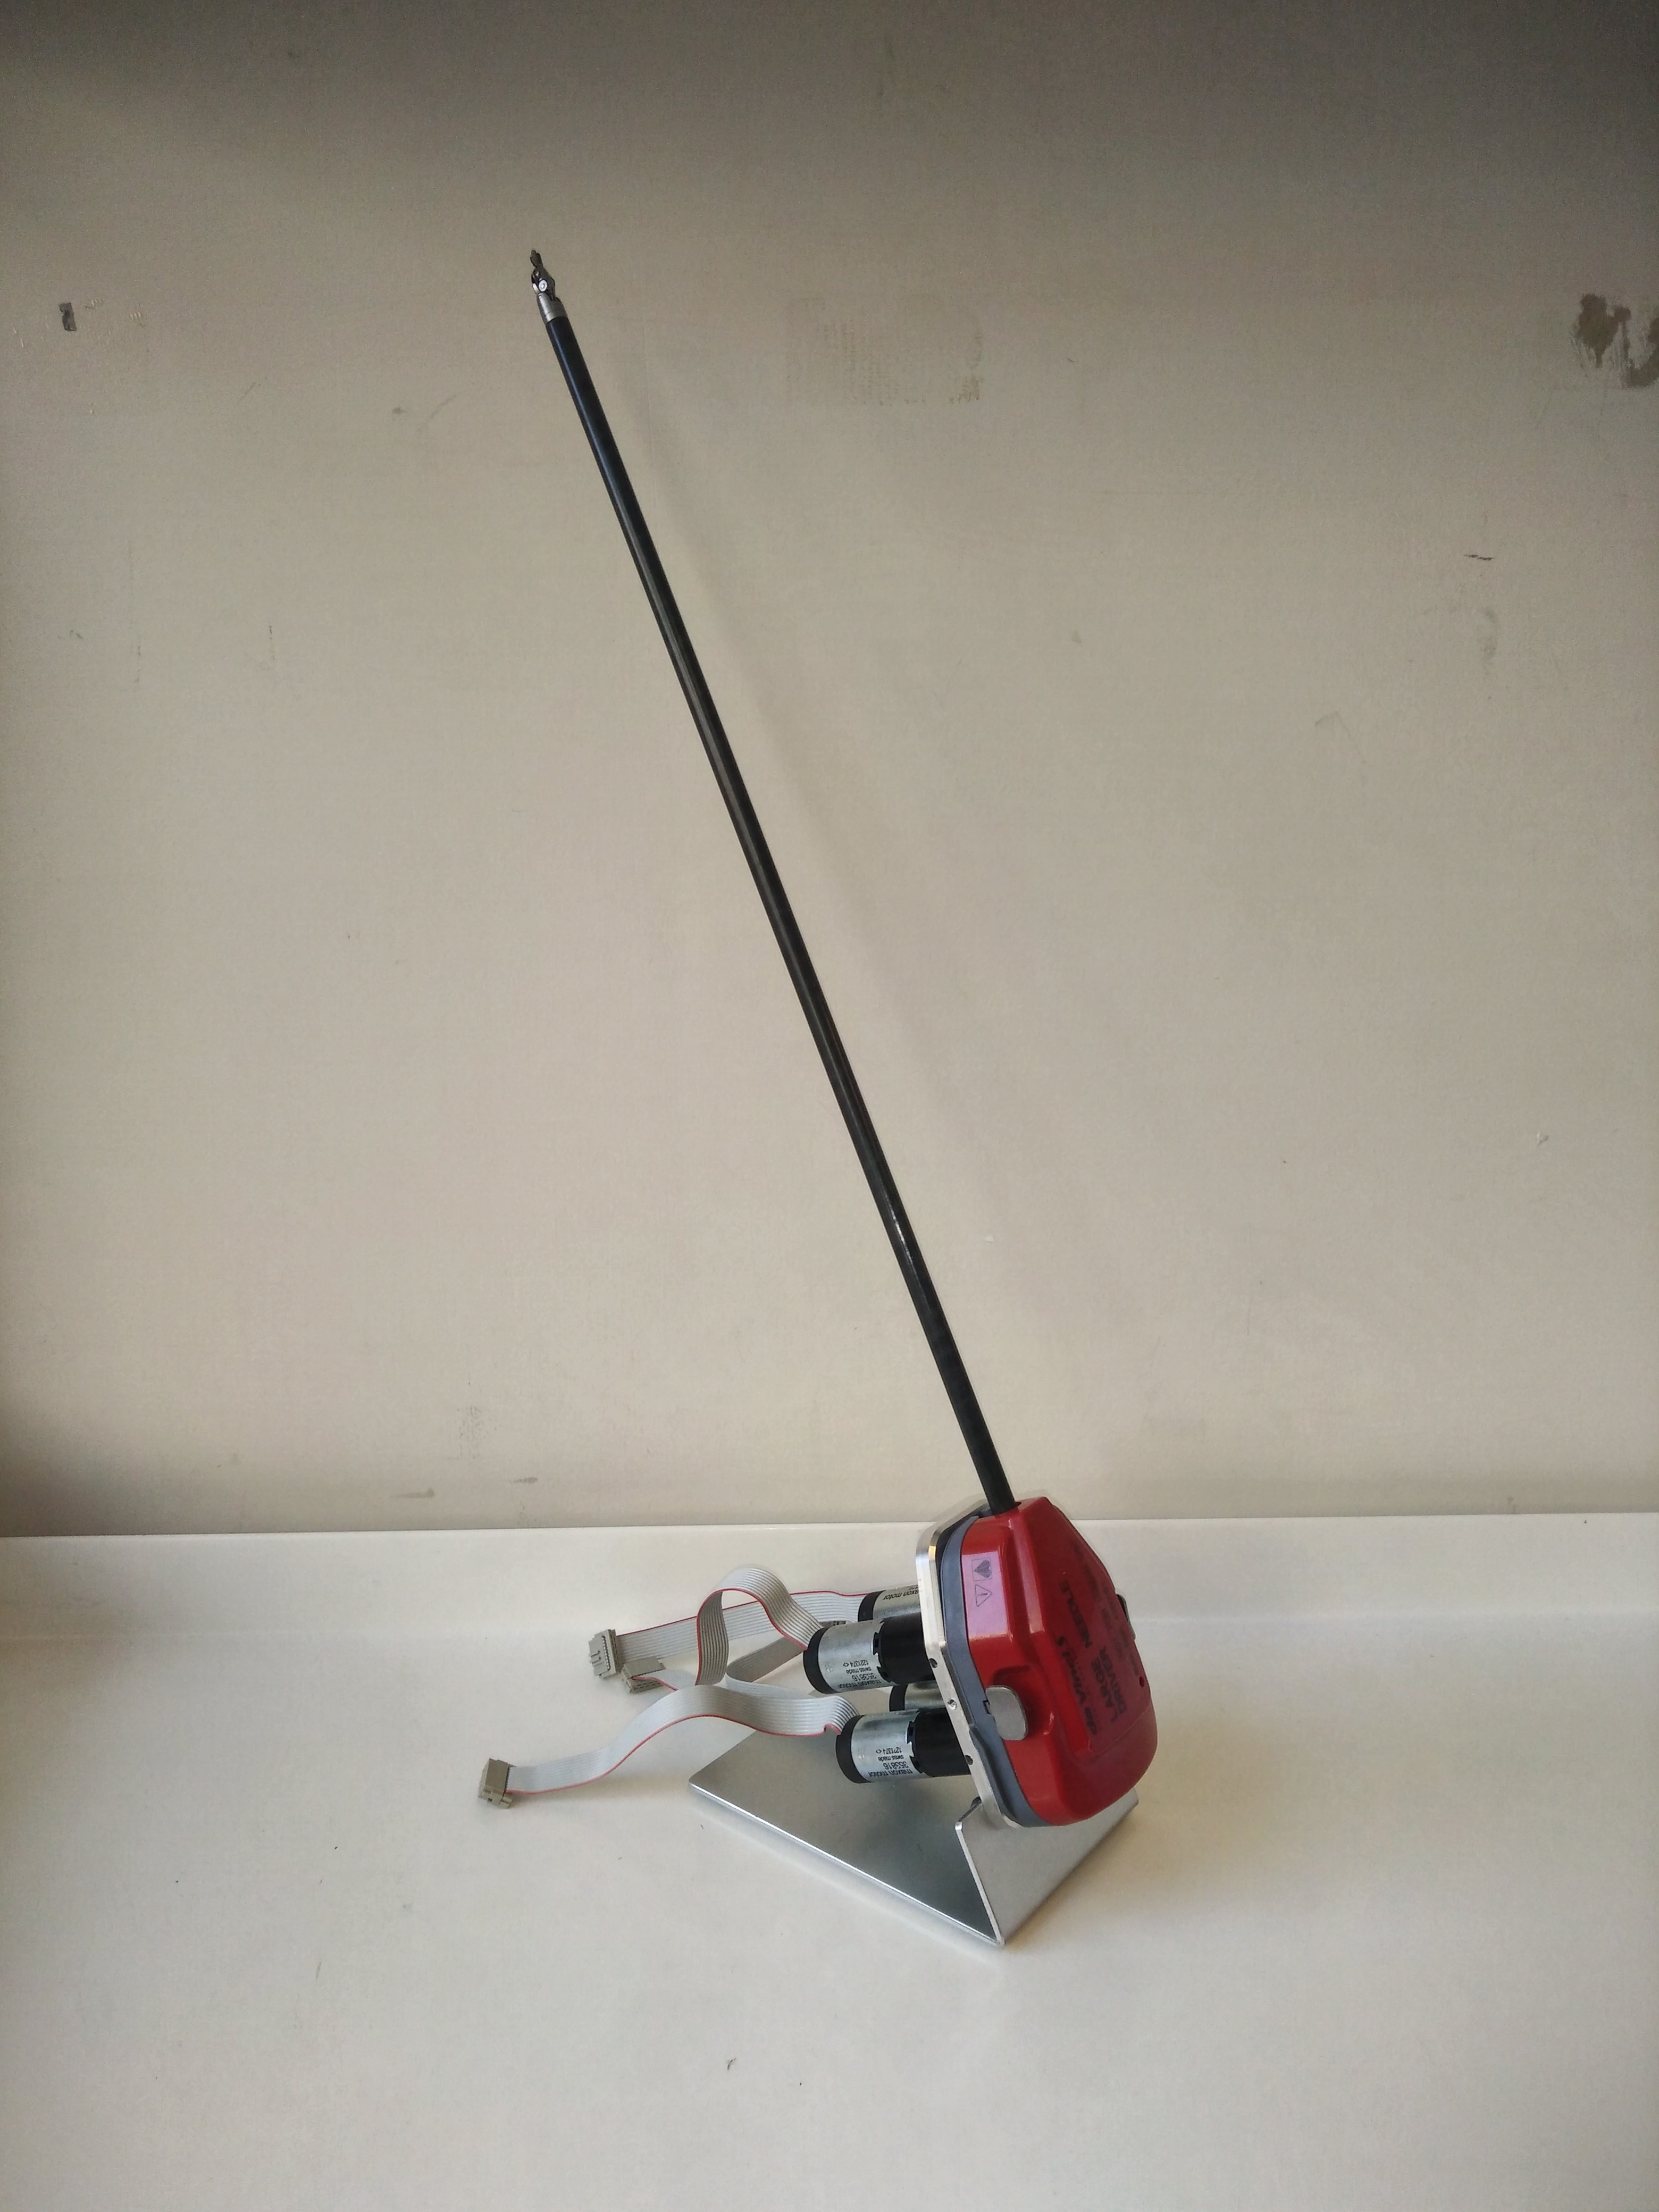
\includegraphics[width=0.4\linewidth]{Test_setup4.jpg}
%     \caption{Full view of the mechanical test setup}
%     \label{fig:Mec_d}
% \end{figure}

% As mentioned before, the sbRio board controls the test setup and as such represents the onboard computer on the DaVinci robot.
% In order to perform higher level functions such as force feedback control, it is necessary to remotely handle data and send high-level commands.
% This is handled by an external computer system that is connected to the Phantom omni device.

% The sbRio board communicates with the computer using UDP \todo{UDP is one of our results and not part of the initial setup} communication protocols, while the Geomagic Touch does so using TCP/IP.
% The computer also performs force estimation using a dynamical model of the test setup (or Endowrist, more precisely), this is vital for force feedback.
% In order to connect software components responsible for communicating with hardware and the ones responsible for the control algorithm and estimation.
% For this purpose we use the Robot Operating System (ROS), which uses a network architecture to share data between components via data streams.

% \begin{figure}[h]
% \centering
% \begin{tikzpicture}
%     % We start by placing the blocks
%     \node [block] (Geomagic) {\small{Geomagic Touch}};
%     \node [block, right of=Geomagic, node distance = 3.4cm] (ROS) {ROS};
%     \node [block, right of=ROS, node distance=3.3cm] (DaVinci) {DaVinci};
%     % We draw an edge between the controller and system block to 
%     % calculate the coordinate u. We need it to place the measurement block. 
%     \draw [<->] (Geomagic) -- node[label=above:\small{TCP/IP}] {} (ROS);
%     \draw [<->] (ROS) -- node [label=above:\small{UDP}] {} (DaVinci);
% \end{tikzpicture}
% \caption{Block diagram representing the system.}
% \end{figure}
